\documentclass[11pt]{article}
\usepackage[sc]{mathpazo} %Like Palatino with extensive math support
% \usepackage{crimson}
\usepackage{fullpage}
\usepackage{amsmath}
\usepackage[normalem]{ulem}
\RequirePackage[authoryear,sectionbib,sort]{natbib}
\bibliographystyle{amnatnat}
\linespread{1.7}
\usepackage{graphicx}
\usepackage[utf8]{inputenc}
\usepackage{lineno}
% \usepackage{titlesec}
% \titleformat{\section}[block]{\Large\bfseries\filcenter}{\thesection}{1em}{}
% \titleformat{\subsection}[block]{\Large\itshape\filcenter}{\thesubsection}{1em}{}
% \titleformat{\subsubsection}[block]{\large\itshape}{\thesubsubsection}{1em}{}
% \titleformat{\paragraph}[runin]{\itshape}{\theparagraph}{1em}{}[. ]\renewcommand{\refname}{Literature Cited}

%%%%%%%%%%%%%%%%%%%%%
% Line numbering
%%%%%%%%%%%%%%%%%%%%%
%
% Please use line numbering with your initial submission and
% subsequent revisions. After acceptance, please turn line numbering
% off by adding percent signs to the lines %\usepackage{lineno} and
% to %\linenumbers{} and %\modulolinenumbers[3] below.
%
% To avoid line numbering being thrown off around math environments,
% the math environments have to be wrapped using
% \begin{linenomath*} and \end{linenomath*}
%
% (Thanks to Vlastimil Krivan for pointing this out to us!)

\title{To be decided: Competition --- movement --- evolution}

% This version of the LaTeX template was last updated on
% November 8, 2019.

%%%%%%%%%%%%%%%%%%%%%
% Authorship
%%%%%%%%%%%%%%%%%%%%%
% Please remove authorship information while your paper is under review,
% unless you wish to waive your anonymity under double-blind review. You
% will need to add this information back in to your final files after
% acceptance.

\author{Pratik R. Gupte$^{1,\ast}$ \\ 
        Christoph F. G. Netz$^{1,\ast}$ \\ 
        Franz J. Weissing$^{1}$}

\date{}

\begin{document}

\maketitle

\noindent{} 1. University of Groningen, Groningen 9747AG, The Netherlands.

\noindent{} $\ast$ Corresponding authors; e-mail: p.r.gupte@rug.nl OR pratikgupte16@gmail.com; c.f.g.netz@rug.nl

\bigskip

\textit{Manuscript elements}: EXAMPLE: Figure~1, figure~2, table~1, online appendices~A and B (including figure~A1 and figure~A2). Figure~2 is to print in color.

\bigskip

\textit{Keywords}: Examples, model, template, guidelines.

\bigskip

\textit{Manuscript type}: Article. %Or e-article, note, e-note, natural history miscellany, e-natural history miscellany, comment, reply, invited symposium, or historical perspective.

\bigskip

\noindent{\footnotesize Prepared using the suggested \LaTeX{} template for \textit{Am.\ Nat.}}

\linenumbers{}
\modulolinenumbers[1]

\newpage{}

\section{Abstract}

To be added.

\section{Introduction}

Competition is a constant feature of animal ecology, and can be an important driver of population dynamics and animal distributions (Krebs 1972; Stephens et al. 2007).
Competition can be broadly classified into two main types, `exploitation' and `interference'. 
In exploitation competition, individuals compete indirectly by depleting a common resource, while in interference competition, individuals compete directly by interacting with each other (Birch 1957; Case and Gilpin 1974; Keddy 2001).
A special case of interference competition which is widespread among animal taxa is `kleptoparasitism', in which an individual steals a resource from its owner (Iyengar et al. 2008; e.g. Furness 1987; Carbone et al. 1997; other examples here).
Experiments with foraging birds have shown that competition, including kleptoparasitism, can affect the spatial distribution of individuals across resource patches (Goss-Custard 1980 Ardea; Vahl et al. 2005a, 2005b, 2007; Rutten et al. 2010a).
The avoidance of competitive interactions too can affect the distribution and behaviour of animals foraging in groups (Bijleveld et al. 2012; Rutten et al. 2010b).
At larger scales, competition among different behavioural types in a species (e.g. Duckworth and Badyayev 2007), or between species (e.g. Petren and Case 1997; Duckworth and Badyayev 2007), can strongly influence species distributions and animal movement decisions (Ovaskainen et al. 2015 MEE; Schlaegel et al. 2020).

Competition is difficult to study in free living animals, yet our knowledge of the fine-scale mechanisms and evolutionary consequences of competition is central to basic evolutionary ecology.
For instance, it is surmised that interference is more important than exploitation under natural conditions (Case and Gilpin 1974, or citations from their first para), but it is difficult to establish whether interference, and especially kleptoparasitism, represents a foraging specialisation shown by part of the population, or whether it is an opportunistic strategy conditioned on local cues, that can be used by all individuals.
Furthermore, it is nearly impossible to study the causes and consequences of competition --- such as its co-evolution with movement strategies, or the effect on resource landscapes --- at evolutionary time-scales in most animals, due to a lack of long-term data (Govaert et al. 2019).
Our poor understanding of competition poses a problem, since it is key to models such as the ideal free distribution concept, which is a cornerstone of evolutionary ecology \citep{fretwell1970}.
The IFD and its developments model competition in quite rudimentary ways \citep{tregenza1995,cressman2006,fretwell1970,meer1997,matsumura2010,amano2006,garay2010,garay2015,garay2020,folmer2012}; IFD-based models ignore resource depletion \citep{fretwell1970,meer1997,cressman2006}, assume unrealistic movement rules \citep{cressman2006,cressman2014,garay2020}, or treat interference as an almost inevitable part of the foraging process \citep[reviewed in][; see also \citealt{cressman2006, garay2020}]{meer1997, tregenza1995}.
On the contrary, interference competition is a complex individual behaviour which is closely related to movement decisions, and its treatment in models is likely to have important ecological and evolutionary consequences \citep{meer1997}.

Modelling competition in a spatially-explicit context, as the outcome of evolved individual movement and behavioural rules, would allow us to (1) better examine the feedbacks between movement and behaviour, and to (2) study the influence of different modelling choices.
Individual-based simulation modelling (IBM) is an increasingly powerful technique that allows us to more realistically model competition among foraging individuals, as well as their interactions with the environment \citep{deangelis2005,deangelis2018,grimm2017,railsback2020,huston1988}.
IBMs take a bottom-up view to encode many thousands of unique individuals with decision making mechanisms, and allow these individuals to interact with their environment, and each other \citep{huston1988,deangelis2019}.
Conceptual and computational advances in IBMs \citep[][]{deangelis2018,deangelis2005} allow us to make general, testable predictions for population-level phenomena \citep[e.g. animal space use, or life-history strategies; see][]{spiegel2017,schaefer2018,folmer2012}, and they are well suited to modelling the evolution of complex behaviours \citep{netz2020,guttal2010,getz2016,getz2015}.

Here, we implement a spatially explicit IBM approach to competition and animal movement decisions, with three different models.
In the first model, we examine how exploitation competition influences the evolution individual movement rules, population level resource intake, and the spatial structure of the resource landscape.
In the second model, we introduce kleptoparasitic interference as an inherited strategy, fixed through an individual's life, and investigate how individual movement and behaviour decisions co-evolve.
In the third model, we model kleptoparasitism more realistically, as a behavioural strategy conditioned on local environmental and social cues, compare the population-level and landscape-scale outcomes between models 2 and 3 to show the influence of modelling choices.
From these models, we show that 1. Foraging with only exploitation competition is usually the most productive strategy from a population standpoint; however an exploitation-only population can be invaded by both fixed and conditional kleptoparasites as kleptoparasitism is the more productive \textit{individual} strategy;
2. The evolution of movement towards successful foragers is an outcome of depleted resource-landscape lacking cues for optimal movement, and is itself a pre-requisite for the persistence of obligate kleptoparasitism;
3. The persistence of kleptoparasitism reduces resource-landscape depletion, and restores cues for optimal movement. 

\section{Methods}

We implement three individual-based evolutionary simulation models whose most basic components --- the environment size and shape, its gridded structure and each cell's capacity to hold multiple individuals, as well as the discrete conception of time within and between generations --- are inspired by \citet{netz2020}.
We conceptualised the models around the behaviour of waders (\textit{Charadrii}, and especially oystercatchers \textit{Haematopus sp.}), which are extensively studied in the context of foraging competition \citep[e.g.][]{vahl2005, vahl2005b, vahl2007, ENS1990219, rutten2010a, rutten2010}.
We simulated a fixed population with a fixed size of 10,000 individuals moving on a landscape of 512\textsuperscript{2} grid cells, with the landscape wrapped at the boundaries so that individuals passing beyond the bounds at one end re-appear on the diametrically opposite side.
Individuals have a lifetime of $T$ timesteps, with $T$ set to 400 by default.
After their lifetime, individuals reproduce and transmit their heritable traits proportional to their fitness over their lifetime.
The model code (in C++) can be found as part of the Supplementary Material in the Zenodo repository at \textbf{Zenodo/other repository here}.

\subsection{Model 1: Exploitative Competition}

The first model simualates only exploitative competition; individuals move about on the landscape and probabilistically find and consume discrete prey items.
Between finding and consuming a prey item, individuals must `handle' the prey for a fixed handling time $T_H$ which is constant across prey items.
Prey handling time $T_H$ is set at 5 timesteps by default.
The handling time dynamic is well known from many systems; for instance, it could be the time required for a wader to break through a mussel shell, with the handling action obvious to nearby individuals, and the prey not fully under the control of the finder.
We refer to such individuals as `handlers' for convenience.
Handlers are assumed to be fully absorbed in their processing of prey, and do not make any movements until they have fully handled and consumed their prey.

\subsection{Models 2 and 3: Kleptoparasitic Intereference Competition}

The second model builds on Model 1, with the addition that individuals inherit a fixed strategy to either forage or to steal prey items from handlers, exclusively.
Agents that steal are termed kleptoparasites.
Kleptoparasites are always successful in stealing from the handler they target; this may be thought of as the benefit of the element of surprise, a common observation among birds \cite{brockmann1979}.
Having acquired prey, a kleptoparasite need only handle it for $T_H - t_h$ timesteps, where $t_h$ is the time that the prey has already been handled by its previous owner; thus kleptoparasites clearly save time on handling compared to a forager.
The targeted handler deprived of its prey is assumed to flee from the area, and does not make a further foraging decision.
Model 3 is similar to model 2, except that individuals process local environmental cues and pick either the forager or kleptoparasite strategy to use in the next timestep.
Apart from the frequency of the choice, the actual foraging dynamics are the same as described in the fixed-strategy case.

\subsection{Movement and Behavioural Strategy}

In all models, individuals use cues available in timestep $t$ to predict their best move for the next timestep $t+1$.
The movement decision is based on three local environmental cues: (1) the number of discrete prey items $F$, (2) the number of individuals handling  prey $H$ (referred to as `handlers'), and (3) the number of individuals not handling prey $K$ (referred to as `non-handlers').
%%
Individuals occupy a single grid cell on the environment at a time, and assign a suitability score $S$ per cell to the nine cells in their Moore neighbourhood as
\begin{linenomath*}
    \begin{equation}
        S = m_fF + m_hH + m_kK
    \end{equation}
\end{linenomath*}
where the weighing factors for each cue $m_f$, $m_h$ and $m_k$ are genetically encoded and heritable between generations.
Individuals rank their Moore neighbourhood by $S$ in timestep $t$ and move to the highest ranked cell in timestep $t+1$.
%%
Individuals in model 1 only forage for prey, while individuals in model 2 either forage or steal based on their inherited strategy.
However, individuals in model 3 process the cell-specific environmental cues $F$, $H$, and $K$ to determine their next foraging strategy as
\begin{linenomath*}
    \begin{equation}
        strategy = 
    \begin{cases}
        {forager},& \text{if } w_fG + w_hH + w_kK + w_b \geq 0\\
        {kleptoparasite},              & \text{otherwise}
    \end{cases}
    \end{equation}
\end{linenomath*}
where the cue weights $f_g$, $f_h$ and $f_p$, and the bias $f_b$ are also genetically encoded and heritable between generations.
Individuals that have been stolen from are an important exception; these `fleeing' individuals are moved to a random cell within a Chebyshev distance of 5, and do not make a foraging decision there.
All individuals move simultaneously, and then implement their foraging or kleptoparasitic behaviour to acquire prey.
Individuals move and forage on the resource landscape for $T$ timesteps per generation, and $T$ is set at 400 by default. 
Handlers are immobile while they process prey for $T_H$ timesteps.

\subsection{Prey Environment and Ecological Dynamics}

\paragraph{Inspiration from Mussel Beds}

Since our model was conceived to represent foraging waders, we developed a resource landscape based on mussels (family \textit{Mytilidae}) that are commonly found in inter-tidal systems.
Mussels (and prey generally) are often less mobile than their consumers, their abundances in the absence of predators are largely driven by external environmental gradients, and they may be frequently found in clusters \citep{dejager2011, dejager2020}.

\paragraph{Prey Abundance}

We modelled relative prey immobility and extrinsically driven abundance by assigning each grid cell of the resource landscape a constant probability of generating a new prey item per timestep, which we refer to as the cell-specific growth rate $r$.
We modelled clustering in the abundance of prey by having the distribution of $r$ across the grid cells take the form of 1,024 uniformly distributed resource peaks with $r$ declining from the centre of each peak (called $r_{max}$) to its periphery (Fig. 1).
Effectively, the cell at the centre of each patch generates a prey item five times more frequently than the cells at the edges.
We ran all three models across a range of $r_{max}$ values (0.001 -- 0.25).
Cells in our landscape were modelled as having a carrying capacity $K$ of 5 prey items, and while a cell is at carrying capacity its $r$ is 0.

\paragraph{Prey Acquisition by Predators}

Individuals can perceive all prey items $G$ in a cell, but have only a probability of finding a prey item $p(success)$.
The $p(success)$ is the probability of not finding any of $F$ prey, each with a detection probability of $p_i$ = 0.2.
\begin{linenomath*}
    \begin{equation}
        p({success}) = 1 - \left(1 - p_i\right) ^ G
    \end{equation}
\end{linenomath*}

As foraging events occur simultaneously, it is possible for more foragers to be considered successful in finding prey than there are discrete items in that cell.
This simple case of exploitation competition is resolved by assigning $F$ prey among some $N$ successful finders at random.
Foragers that are assigned a prey item in timestep $t$ begin handling it, and are considered to be handlers for the purposes of timestep $t+1$, i.e., movement and foraging decisions of other individuals).
Foragers that are not assigned a prey item are considered idle during timestep $t$, and are counted as non-handlers for $t+1$.

Kleptoparasites successfully steal from a handler, contingent on the number of handlers matching or exceeding the number of kleptoparasites in timestep $t$.
When the number of kleptoparasites exceeds handlers, handlers are assigned among kleptoparasites at random.
Successful kleptoparasites convert into handlers.
Unsuccessful kleptoparasites are considered idle, and are also counted as non-handlers for timestep $t+1$.
Handlers that finish processing their prey in timestep $t$ return to the non-handler state and are assessed as such by other individuals when determining movements for $t+1$.

\subsection{Reproduction and the Evolution of Decision Making}

At the end of each generation, the population is replaced by its offspring, maintaining a fixed population size. 
The decision-making weights which determine individual movement ($m_f$, $m_h$, $m_k$) and foraging strategy choice ($w_f$, $w_h$, $w_k$, $w_b$) are transmitted from parent individuals to offspring.
The total lifetime intake of individuals is used as a proxy of fitness.
%%
The number of offspring of each parent is thus proportional to the parent's share of the population intake, and this is implemented as a weighted lottery that selects a parent for each offspring.
The decision-making weights are subject to independent random mutations with a probability of 0.001.
The size of the mutation (either positive or negative) is drawn from a Cauchy distribution with a scale of 0.01 centred on the current value of the weight to be mutated.
This allows for a small number of very large mutations while the majority of mutations are small.
%%
We recognised that spatial autocorrelation in the landscape coupled with limited natal dispersal can lead to spatial heterogeneity in evolved movement rules, as lineages adapt to local conditions \citep[][]{wolf2010}.
Furthermore, limited natal dispersal could lead to population-level movements due to differential reproduction that mirror shifts in resource abundance, rather than individual movement rules.
To ensure that global individual movement rules evolved, we intialised each offspring at a random location on the landscape, and also reset its total intake to zero.

\subsection{Simulation Output and Analysis}

\paragraph{Population Activities and Individual Decisions}

We counted the number of times the forager or kleptoparasite strategy was used in each generation of our simulations, as well as the number of times no strategy could be used because individuals were handling a food item.
We refer to the ratio of time spent foraging, stealing, and handling as the population's `activity budget'.
We examined how the population activity budget developed over evolutionary time, and whether a stable ecological equilibrium was reached.
Furthermore, we counted the total population intake --- the number of items consumed in each generation --- as a measure of population productivity.
%
To understand the evolutionary consequences of our simulation on the individual decision making weights, we exported the weights of each individual in every generation of the simulation.

\paragraph{Changes in the Resource Landscape}

Anticipating that the prevalence of different foraging strategies would affect the spatial structure of the prey-item landscape, we examined changes in the prey-item abundances of landscape grid cells.
We exported a snapshot of the the number of items per grid-cell at the mid-point of each generation ($t$ = 200), for each simulation run, and we visually examined how landscape patterns changed over generations.
%%
We then addressed a specific question: how would the ability of individuals to navigate their landscape change with the reduced depletion expected with kleptoparasitism?
Individuals can only choose an optimal move when they can sense profitability differences (such as the number of prey-items) among the various destinations.
We quantified the cell-specific item gradient for each landscape snapshot, and determined the difference in items between each cell and its neighbours (the item gradient).
We calculated the proportion of the landscape that formed a `clueless plateau', i.e., where the item gradient was zero (\textit{sensu} \citealt{perkins1992a}).

\paragraph*{Data Availability}

Simulation data used in this study are available on the Dryad/IRODS/Zenodo repository \textbf{REPOSITORY LINK HERE}; 
simulation code is available on Github and archived on Zenodo at \textbf{ZENODO LINK HERE}; 
data analysis and figure code is available on Github and archived on Zenodo at \textbf{ZENODO LINK HERE}.

\section{Results}

\subsection{Model Outcomes}

All three models result in population level activity budget equilibria with stable proportions of foraging, kleptoparasitism, and handling (see Fig. 2A, 3A, 4A).
Populations reach this stable state within 100 generations, i.e., 10\% of evolutionary time.
Once a population reaches an activity budget equilibrium, it also reaches an intake equilibrium which is closely related to the proportion of handling (Figure 2B, 3B, 4B).

\paragraph{Model 1: Exploitative Competition}

In Model 1, the population's activities is split among foraging and handling (Fig. 2A; $r_{max}$ = 0.01).
The proportion of handling in the activity budget, and the population intake are both initially low, but then peak within ten generations (Fig. 2B).
This is because individuals can easily acquire prey items from the fully stocked landscape in the first few generations.
As individuals deplete prey items faster than they can be replenished, the overall number of prey items is reduced (Fig. 2C).
Population handling activity declines to a stable value $\sim$ 45\% within 50 generations, leading to a similar stabilisation in population intake (Fig. 2A, 2B).
The number of individuals per cell declines between generations one and fifty (Fig. 2C).

\paragraph{Model 2: Interference as a Fixed Strategy}

In Model 2, the population activity budget comprises of foraging, handling, and stealing (Fig. 3A; $r_{max}$ = 0.01).
Population handling and intake shows an initial spike similar to Model 1 as individuals successfully acquire prey items from the fully stocked prey landscape, but then declines to a stable value within 50 generations (Fig. 2A, 2B).
The proportion of individuals with an inherited kleptoparasitic strategy, initially 50\%, declines rapidly to nearly none within the first couple of generations. 
However, after this initial crash, kleptoparasitic individuals rise in frequency to a stable $\sim$70\% of the population (Fig. 3A).
This is reflected in the activity budget, in which stealing rises from nearly zero to form $>$ 50\% of all activities; this is associated with a stabilisation of the proportion of handling at $>$ 25\% (Fig. 3A).
This lower proportion of handling results in lower population intake (Fig. 3B), and a strong \textit{increase} in the number of prey items on the landscape (Fig. 3C).
The number of individuals per cell does not change significantly between generations one and fifty (Fig. 3C).

\paragraph{Model 3: Interference as a Conditional Strategy}

In Model 3, the activity budget is quite different from either Models 1 or 2.
Handling is the most common activity ($\sim$45\%) as in Model 1, with the remaining activities split evenly between foraging and stealing, and a stable equilibrium within 50 generations (Fig. 4A; $r_{max}$ = 0.01).
However, unlike Model 2, the frequency of stealing does not strongly track the frequency of individuals which would show a kleptoparasitic response to handlers (i.e., nearly all individuals within 50 generations; Fig. 4A).
Population intake stabilises within ten generations to a level similar to Model 1 (Fig. 4B).
The reduced depletion following the evolution and persistence of kleptoparasitism leads to landscape change intermediate between Models 1 and 2 within 50 generations; the number of individuals per cell is also reduced (Fig. 4C).

\subsection{The Effect of Landscape Productivity}

The landscape's $r_{max}$ has a marked effect on population activity budgets and total intake.
The frequency of foraging reduces with $r_{max}$ in Models 1 and 3; this is caused by more frequent acquisition of prey items (as regrowth keeps pace with depletion), which results in a greater frequency of handling rather than foraging.
In Model 2 however, the frequency of handling is relatively unaffected by increasing $r_{max}$ (Fig. 5A).
The difference between Models 2 and 3 has to do with the change in the frequency of kleptoparasitism (Fig. 5B).
In Model 2, kleptoparasitism forms $>$ 75\% of all activities at very low $r_{max}$, and is much more common than in Model 3 populations at the same regrowth rate.
However, at relatively high $r_{max}$ (0.03), the fixed kleptoparasitic strategy goes extinct.
At these regrowth rates, the Model 2 population matches the Model 1 population, with foragers rapidly converted to handlers.
In Model 3, kleptoparasitism persists at low frequencies even at the highest regrowth rates (Fig. 5B); thus some foragers lose time in extracting items which are then stolen from them.
Consequently, while populations in all three models achieve very similar intakes at low $r_{max}$, at intermediate regrowth rates (0.01 -- 0.025), conditionally kleptoparasitic populations outperform populations using fixed strategies.
Only at high regrowth rates, when fixed strategy populations (Model 2) effectively convert to purely forager populations (Model 1), do they achieve a higher intake than Model 3 populations (Fig. 5C).

\subsection{The Evolutionary and Ecological Consequences of kleptoparasitism}

The evolution and persistence of kleptoparasitism reduces prey-item depletion compared to the foragers-only case, and allows many localised gradients of prey-item abundance to re-emerge (Figs. 2C, 3C, 4C).
In Model 1, depletion reaches a stable value, and the proportion of the landscape with no item cues (`clueless plateaus') follows it to a stable level of 75\% by generation 10 ($r_{max}$ = 0.01; Fig. 6A, 6D).
Consequently, forager individuals slowly evolve to move towards handlers (blue line; Fig. 6A), as the presence of a handler marks a cell as having a non-zero probability of generating a prey item.
%
In model 2, clueless plateaus comprise $>$ 50\% of the landscape by generation 10, but then rapidly subside to $<$ 25\% by generation 20, following rapid reductions in resource landscape depletion (Fig. 6B, 6E).
As most individuals are kleptoparasites (orange line; Fig. 6B), and moving towards handlers is the only viable kleptoparasite movement strategy, the population as a whole evolves to move towards handlers (blue line; Fig. 6B).
%%
In Model 3, depletion stabilises at a value intermediate between Models 1 and 2, and, clueless plateaus stabilise at $\sim$50\% of the landscape (Fig. 6C, 6F).
Model 3 individuals are faced with both a lesser abundance of prey-items than in model 2, as well as being able to steal from any handlers they encounter; as a consequences, all individuals evolve a preference for moving towards handlers (blue line; Fig. 6C), which represent both a direct resource as well as an indication of prey item abundance.

When kleptoparasitism is a fixed, inherited strategy (model 2), kleptoparasitic individuals face a particularly strong selection pressure to move towards handlers, as these are their only food source (Fig. 7A).
As kleptoparasites form an increasing proportion of the population, they also form an increasing proportion of individuals with a preference for moving towards handlers (Fig. 7B).
In contrast, foragers are largely neutral to handlers, and as they decrease in frequency, they form a decreasing proportion of individuals with a preference for handlers (Fig. 7A, 7B).

\section{Discussion}

short summary of results?

\subsection{Exploitation Competition Does Not Produce Polymorphisms}

Competition is a key process in determining animal space use across scales, and can lead to the diversification of populations as individuals specialise to avoid competition.
Here, we show how the mechanisms of competition and movement are key to this diversification.
In our Model 1 with only exploitative competition, only a single movement morph evolves.
Previous models of the evolution of movement rules suggest that multiple movement morphs should evolve in a forager-resource context \citep[][Netz et al. in prep.]{getz2015}.
However, both models include two components missing from Model 1: interference competition, and movement costs, highlighting the insufficiency of exploitative competition alone to generate phenotypic polymorphisms.

\subsection{Polymorphism as the Outcome of Constraints}

Our Models 2 and 3 further show how constraints, such as a movement or strategy cost, are key to the evolution of polymorphisms.
In our Model 2, the modelling of kleptoparasitic interference as a fixed strategy leads to the dimorphism between obligate foragers and kleptoparasites.
This constraint is resolved in Model 3, and individuals evolve to be kleptoparasitic in the presence of handlers, and foragers otherwise.
The strategy constraint on Model 2 individuals prevents the population from converging on a single behavioural and movement phenotype, as kleptoparasites are dependent on foragers for intake.

Fixed-strategy populations evolve a further polymorphism in movement behaviour, with kleptoparasites moving towards handlers, and foragers neutral to handlers.
This coupling of movement and behavioural strategy is expected because obligate kleptoparasites functionally occupy a higher trophic level whose primary resource is handling foragers, rather than prey items.
Once the the handler-preference in fixed in kleptoparasitic lineages, it becomes the more frequent handler response (over avoidance) as kleptoparasites increase in frequency.

Several factors contribute to the stabilisation of kleptoparasitism at high frequencies, rather than the emergence of limit cycles of kleptoparasites and foragers.
Among the most important is global natal dispersal, which ensures a well-mixed population in each generation, rather than increasing densities of offspring (of either strategy) around the most successful ancestors (`differential reproduction').
Differential reproduction would allow instabilities related to spatial structuring, whereby increasing  kleptoparasite density in an area would eventually lead to lower per-capita intake among kleptoparasites relative to foragers, and consequently an increase in the forager:kleptoparasite ratio.

\subsection{Plasticity, Polymorphisms, and Productivity}

Model 3, which allows individuals to opportunistically steal prey items, resolves the strategic constraint of Model 2.
When the inherited decision making weight is conditionally coupled with expressed behaviour, the frequency of stealing attempts better reflects the encounter rate of handlers, rather than the frequency of stealing propensity in the population.
Model 3 individuals' behaviour is thus more adapted to immediate, local conditions; they lose less time in futile stealing attempts, and thus achieve better intakes.
Consequently, individuals rapidly converge upon a single, optimal strategy, which is to steal when handlers are available, and to forage otherwise.

Conditional strategy populations thus outperform fixed-strategy populations, and have similar intakes as forager populations, on low productivity landscapes.
On more productive landscapes ($r_{max} \geq$ 0.02), exploitation competition is reduced, and the probability of a forager-prey item encounter is much higher than the probability of a kleptoparasite-handler encounter.
Consequently, fixed-strategy kleptoparasites rarely match the per-capita intakes of foragers, and rapidly go extinct.
Thus high $r_{max}$ instances of Model 2 consistently produce populations that are functionally identical to Model 1 populations, with no kleptoparasitism.
However, at high $r_{max}$, opportunistic kleptoparasites in Model 3 have a greater per-capita intake rate than pure foragers, as kleptoparasitic prey acquisition deprives a (foraging) handler of its prey. 
This allows kleptoparasitic interference to persist, while also resulting in slightly lower total population intake than the pure forager populations of Model 1 and high $r_{max}$ Model 2.

\subsection{Competition and Landscape Effects}

Competition strongly influences landscape structure, which has cascading ecological and evolutionary effects.
In Model 1, foragers face exploitation competition alone, and rapidly deplete prey items, which results in a large, stable proportion of the landscape forming clueless plateaus, with few movement cues \citep{perkins1992a}.
Consequently, individuals slowly converge upon a movement strategy that makes use of public information in the form of handling individuals, which indicate a non-zero prey-item generation probability.
%%
In Model 2, the emergence and persistence of kleptoparasitism at low $r_{max}$ reduces resource depletion, prey-items are regenerated, and the proportion of clueless plateaus is reduced.
Ironically, the abundance of item cues is not functionally useful to most individuals; kleptoparasites find themselves in a `desert of plenty' as their only resource is handlers, which are uncommon relative to prey items.
On the other hand, for foragers, which can only handle one prey-item at a time, moving at random becomes a viable strategy once most cells have at least one prey-item.
%%
Model 3 populations evolve kleptoparasitism, which similarly depresses prey-item depletion, and reduces the proportion of clueless plateaus.
However, due to their conditional strategies, these individuals make use of the full range of cues for movement and behaviour decisions.


1. exploitation is not sufficient to cause morphs without costs on movement strategy? movement distance? basically without negative density dependence (costs are super important).

2. in model 2, there are behavioural morphs because of imposed constraints, ie, individuals have a fixed strategy. refer to examples.

2.5. model 2: foragers persist because they are  necessary to the system. klepts persist at some growth rates because stealing is the more profitable individual strategy at low growth rates.

2.6. model 2: klepts and foragers both evolve nh-avoidance and item preference as these are heavily conserved traits.

2.7. model 1: ephemeral information beacons on uninformative landscape, sociability OR assessing individual condition is important when there are few other cues

3. Model 3 resolves the constraint through context-dependent behavior, in which case the polymorphism vanishes.

4. klepts reduce resource depletion, act as third trophic level.
something something landscape of fear

% Yet movement behaviour leaves few clues as to its origins, and its long-term effects on populations and landscapes are yet more challenging to measure at an evolutionary scale.
% The proximate, ecological causes and consequences of animal movement are now understood in unprecedented detail, but the ultimate causes and large-scale consequences are poorly understood.
% Animals, moving in response to internal and external stimuli, are key components of their ecosystems \citep{nathan2008,jeltsch2013}.
% The consequences of myriad individual movement responses to local environmental cues result in large-scale emergent phenomena such as population distributions, community assembly, and landscape change \citep{jeltsch2013,schlagel2020}.
% For instance, variation in dispersal movements between two species of bluebird \textit{Sialia sp.}, caused by differences in aggressiveness, results in unexpected cascading effects on inter-specific competition for habitat, and consequently on community composition \citep{duckworth2007}.
% Similarly, there are strong feedbacks between the movement of consumers and their landscapes; while megafauna such as American bison \textit{Bison bison} engineer their ecosystems by facilitating plant growth and nutrient transfer \citep[][]{geremia2019,geremia2020,leroux2018}, predators can structure the same landscapes indirectly by affecting the movement of herbivores \citep[the landscape of fear;][]{leroux2018,kohl2018,brown1999}.

% However, the oversimplification of both consumer-resource dynamics and the evolution of movement strategies \citep[e.g.][]{cressman2006} make for serious conceptual shortcoming. --- move to discussion
% We already know that resource consumption by (mobile) animals can in some cases facilitate the regeneration of these resources \citep[][; see also \citealt{kotanen2013}]{geremia2019,leroux2018}, while in others catastrophically degrading them \citep{siero2019,koppel2008,dekoppel1997,kotanen2013}. --- move to discussion
% A population's evolutionary history on a landscape is also likely to shape individual responses to environmental cues at ecological timescales, as these are mostly drawn from a repertoire transmitted between generations. --- move to  discussion
% For instance, ungulate populations occupying a habitat for generations track resource waves better than those recently translocated into a novel habitat, as resource tracking improves over evolutionary time \citep[][]{jesmer2018}. --- move to discussion also

% For instance, \citeauthor{getz2015}'s (2015, 2016) work models unrealistic evolutionary processes, and \citeauthor{netz2020}'s multi-trophic model yields complex dynamics in which eco-evolutionary processes are difficult to disentangle. --- move to discussion

Ssomething about klepts allowing landscape regrowth --- similar to predation --- landscape of fear etc etc


\section{Conclusion}


%%%%%%%%%%%%%%%%%%%%%
% Acknowledgments
%%%%%%%%%%%%%%%%%%%%%
% You may wish to remove the Acknowledgments section while your paper 
% is under review (unless you wish to waive your anonymity under
% double-blind review) if the Acknowledgments reveal your identity.
% If you remove this section, you will need to add it back in to your
% final files after acceptance.

\section{Acknowledgments}

The authors thank Hanno Hildenbrandt for contributing extensively to the coding of the simulation model \textit{Kleptomove};
Matteo Pederboni for contributing to the model's development; 
and members of the Modelling Adaptive Response Mechanisms Group, and of the Theoretical Biology department at the University of Groningen for helpful discussions on the manuscript.

\bibliography{kleptomove}

\newpage{}

\section{Appendix A: Supplementary Figures}

% In many cases, The American Naturalist allows authors to typeset 
% their own supplementary material in an author-supplied PDF. For author-
% supplied PDFs, please consult the AmNat_supp_template.tex document,
% available from https://www.journals.uchicago.edu/journals/an/instruct 
%
% By contrast, the Appendix instructions below apply to cases in which
% supplementary material is to be typeset by the AmNat editorial staff.
% That notably includes descriptions of methods, tables defining parameters,
% and other material necessary for reproducing the MS's results.
%
% Please reset counters for the appendix (thus normally figure A1, 
% figure A2, table A1, etc.).
%
% In certain cases, it may be appropriate to have a PRINT appendix in
% addition to (or instead of) an online appendix. In this case, please 
% name the print appendix Appendix A, and any subsequent appendixes (if 
% there are any) should be named Online Appendix B, Online Appendix C,
% etc.
%
% Counters for each appendix should match the letter of that appendix.
% For example, tables in Appendix C should be numbered table C1, table C2,
% etc. This applies to tables, equations, and figures.
%
% It's better not to use the \appendix command, because we have some
% formatting peculiarities that \appendix conflicts with.

\renewcommand{\theequation}{A\arabic{equation}}
% redefine the command that creates the equation number.
\renewcommand{\thetable}{A\arabic{table}}
\setcounter{equation}{0}  % reset counter 
\setcounter{figure}{0}
\setcounter{table}{0}

\subsection{Fox--dog encounters through the ages}

% The quick red fox jumps over the lazy brown dog. The quick red fox has always jumped over the lazy brown dog. The quick red fox began jumping over the lazy brown dog in the 19th century and has never ceased from so jumping, as we shall see in figure~\ref{Fig:Jumps}. But there can be surprises (figure~\ref{Fig:JumpsOk}).

% If the order and location of figures is not otherwise clear, feel free to include explanatory dummy text like this:

% [Figure A1 goes here.]

% [Figure A2 goes here.]

% \subsection{Further insights}

% Tables in the appendices can appear in the appendix text (see table~\ref{Table:Rivers} for an example), unlike appendix figure legends which should be grouped at the end of the document together with the other figure legends.

% \begin{table}[h]
% \caption{Various rivers, cities, and animals}
% \label{Table:Rivers}
% \centering
% \begin{tabular}{lll}\hline
% River        & City        & Animal            \\ \hline
% Chicago      & Chicago     & Raccoon           \\
% Des Plaines  & Joliet      & Coyote            \\
% Illinois     & Peoria      & Cardinal          \\
% Kankakee     & Bourbonnais & White-tailed deer \\
% Mississippi  & Galena      & Bald eagle        \\ \hline
% \end{tabular}
% \bigskip{}
% \\
% {\footnotesize Note: See table~\ref{Table:Founders} below for further table formatting hints.}
% \end{table}

% Lorem ipsum dolor sit amet, as we have seen in figures~\ref{Fig:Jumps} and \ref{Fig:JumpsOk}.

\newpage{}
\renewcommand{\theequation}{B\arabic{equation}}
% redefine the command that creates the equation number.
\renewcommand{\thetable}{B\arabic{table}}
\setcounter{equation}{0}  % reset counter 
\setcounter{table}{0}

\section{Appendix B: Additional Methods}

\subsection{Measuring the height of fox jumps without a meterstick}

% Pellentesque ac nibh placerat, luctus lectus non, elementum mauris. 
% Morbi odio velit, eleifend ut hendrerit vitae, consequat sit amet 
% nulla. Pellentesque porttitor vitae nisl quis tempus. Pellentesque 
% habitant morbi tristique senectus et netus et malesuada fames ac 
% turpis egestas. Praesent ut nisi odio. Vivamus vel lorem gravida 
% odio molestie volutpat condimentum et arcu (\citealt{tytler-mqos}). 

% \begin{equation}
% { \frac{1}{N_k-1} \sum \limits_{t=1}^{N_k} (M_{tjk} - \bar{M}_{jk})^2}
% \end{equation}

% \subsection{Quantifying the brownness of the dog}

% Pellentesque eu nulla odio (\citealt{Xiao2015,CookEtAl2015}). Nulla aliquam porta metus, quis malesuada orci faucibus quis. Suspendisse nunc magna, tristique sit amet sollicitudin nec, elementum et lacus. Sed vitae elementum mi. In hac habitasse platea dictumst. Etiam eu tortor elit. Sed ac tortor purus. Aliquam volutpat, odio sit amet posuere pretium, dolor ex interdum ante, sed luctus quam eros ac nulla. 

% \begin{equation}
% { (\sum \limits_{p=1}^P {n_{sp}})^{-1}\sum \limits_{p=1}^P {n_{sp}Q_{p}}}
% \end{equation}

\newpage{}

%%%%%%%%%%%%%%%%%%%%%
% Bibliography
%%%%%%%%%%%%%%%%%%%%%
% You can either type your references following the examples below, or
% compile your BiBTeX database and paste the contents of your .bbl file
% here. The amnatnat.bst style file should work for this---but please
% let us know if you run into any hitches with it!
%
% If you upload a .bib file with your submission, please upload the .bbl
% file as well; this will be required for typesetting.
%
% The list below includes sample journal articles, book chapters, and
% Dryad references.

\newpage{}

\section{Tables}
\renewcommand{\thetable}{\arabic{table}}
\setcounter{table}{0}

% \begin{table}[h]
% \caption{Founders of \textit{The~American Naturalist}}
% \label{Table:Founders}
% \centering
% \begin{tabular}{lll}\hline
% Early editor            & Years with the journal \\ \hline
% Alpheus S. Packard Jr.  & 1867--1886 \\
% Frederick W. Putnam     & 1867--1874 \\ 
% Edward S. Morse         & 1867--1871 \\ 
% Alpheus Hyatt           & 1867--1871 \\
% Edward Drinker Cope$^a$ & 1878--1897 \\
% J.~S. Kingsley          & 1887--1896 \\ \hline 
% \end{tabular}
% \bigskip{}
% \\
% {\footnotesize Note: Table titles should be short. Further details should go in a `notes' area after the tabular environment, like this. $^a$ Published the first description of \textit{Dimetrodon}.}
% \end{table}

\newpage{}

\section{Figure legends}

\begin{figure}[h!]
    \centering
    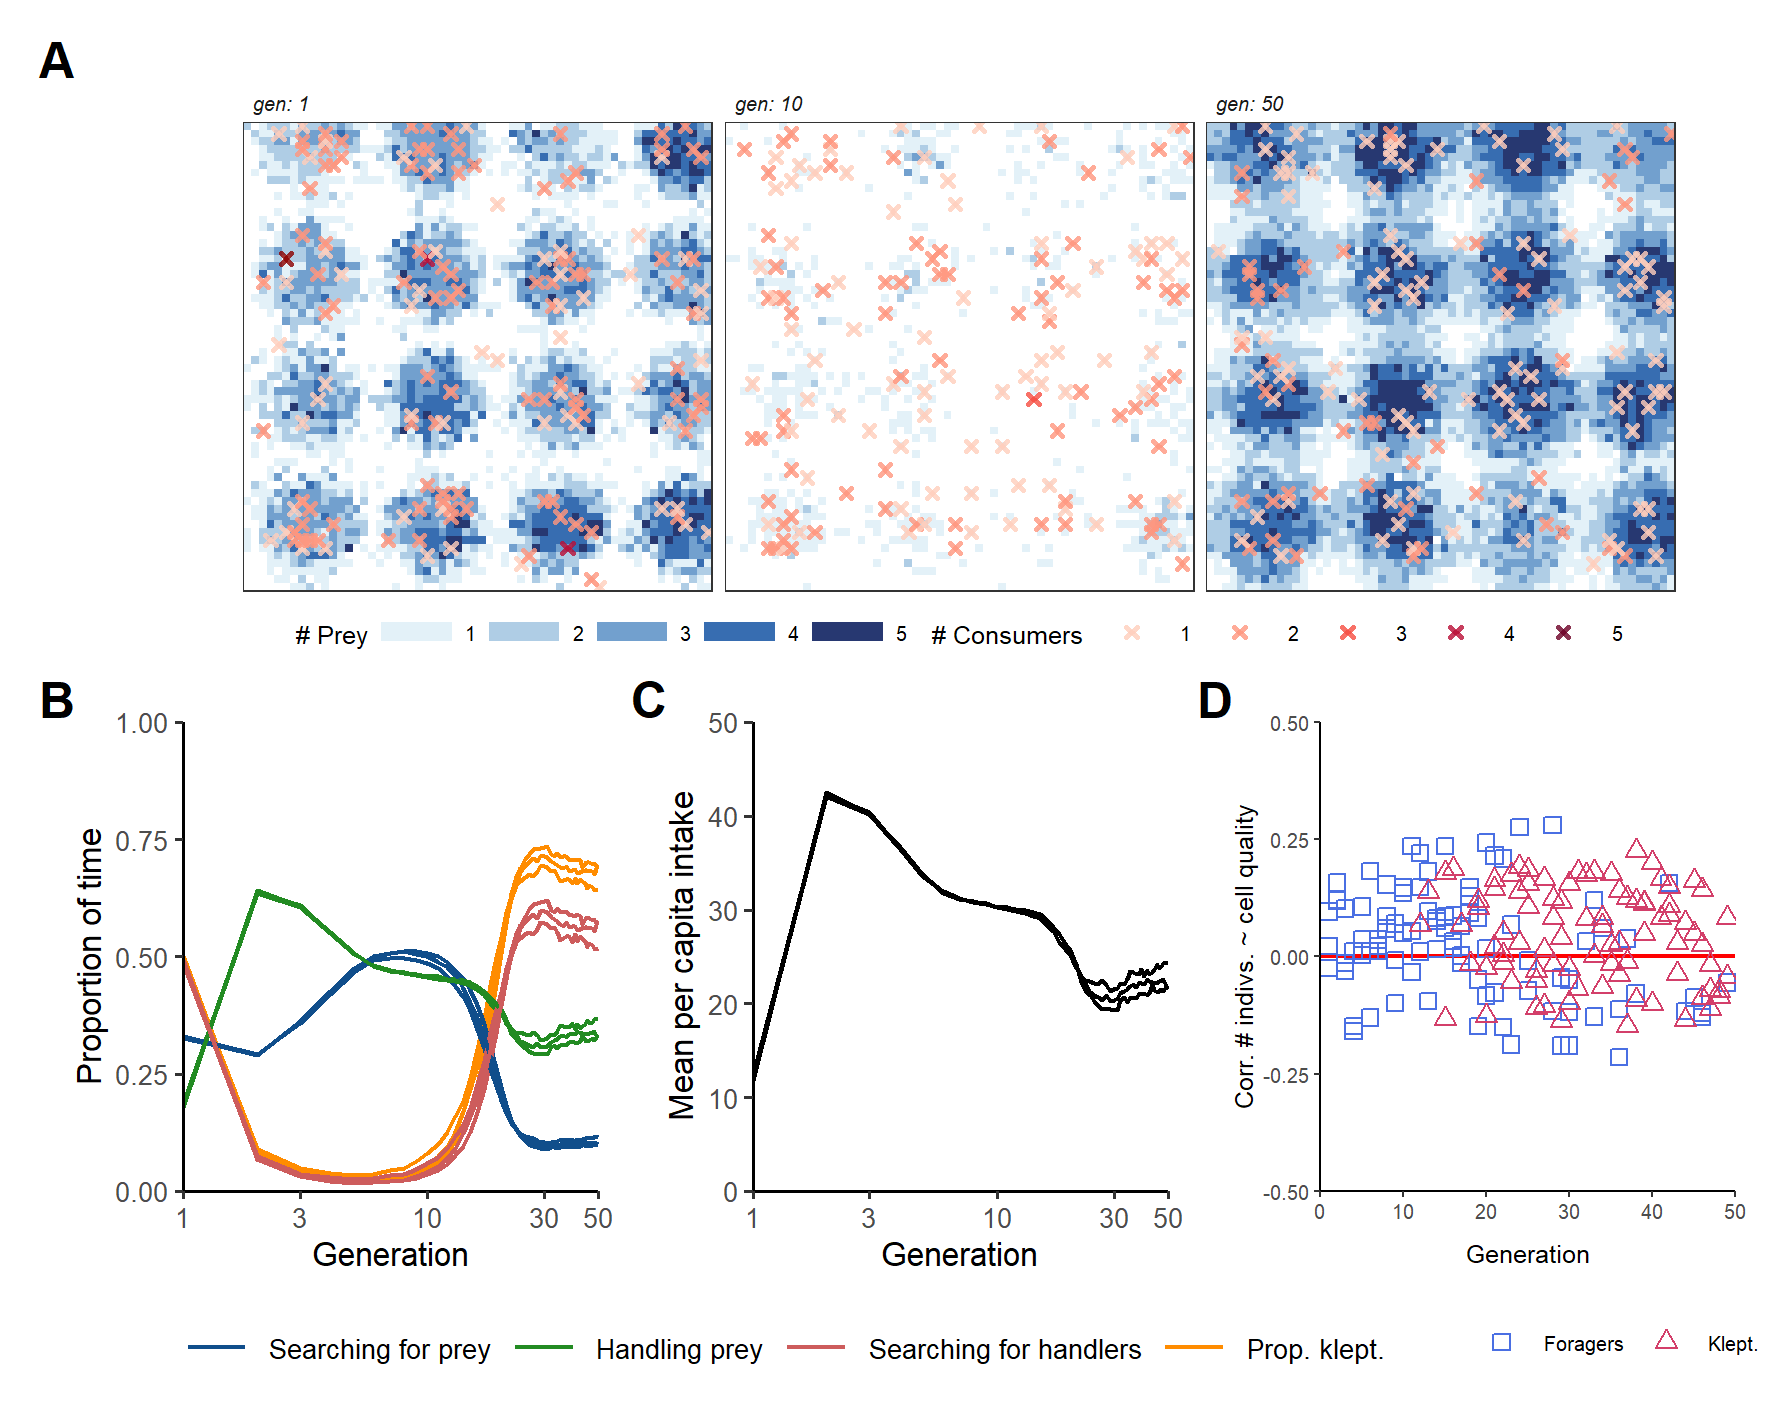
\includegraphics[width=0.85\textwidth]{figures/fig_02.png}
    \caption{
        Model 1 populations with only exploitation competition rapidly reach an \textbf{(A)} activity budget and \textbf{(B)} total intake equlibrium. The initial spike in handling and population intake is due to initially high foraging success on a fully stocked resource landscape.
        \textbf{(C)} The sustained extraction of prey-items results in a rapid depletion of the resource landscape within 50 generations. The number of individuals on occupied cells is shown as black circles (size = number of individuals). Panels \textbf{A, B} show three replicates, while panel \textbf{C} shows a single replicate; all panels are for $r_{max}$ = 0.01.
    }
    \label{Fig:Model1}
\end{figure}

\begin{figure}[h!]
    \centering
    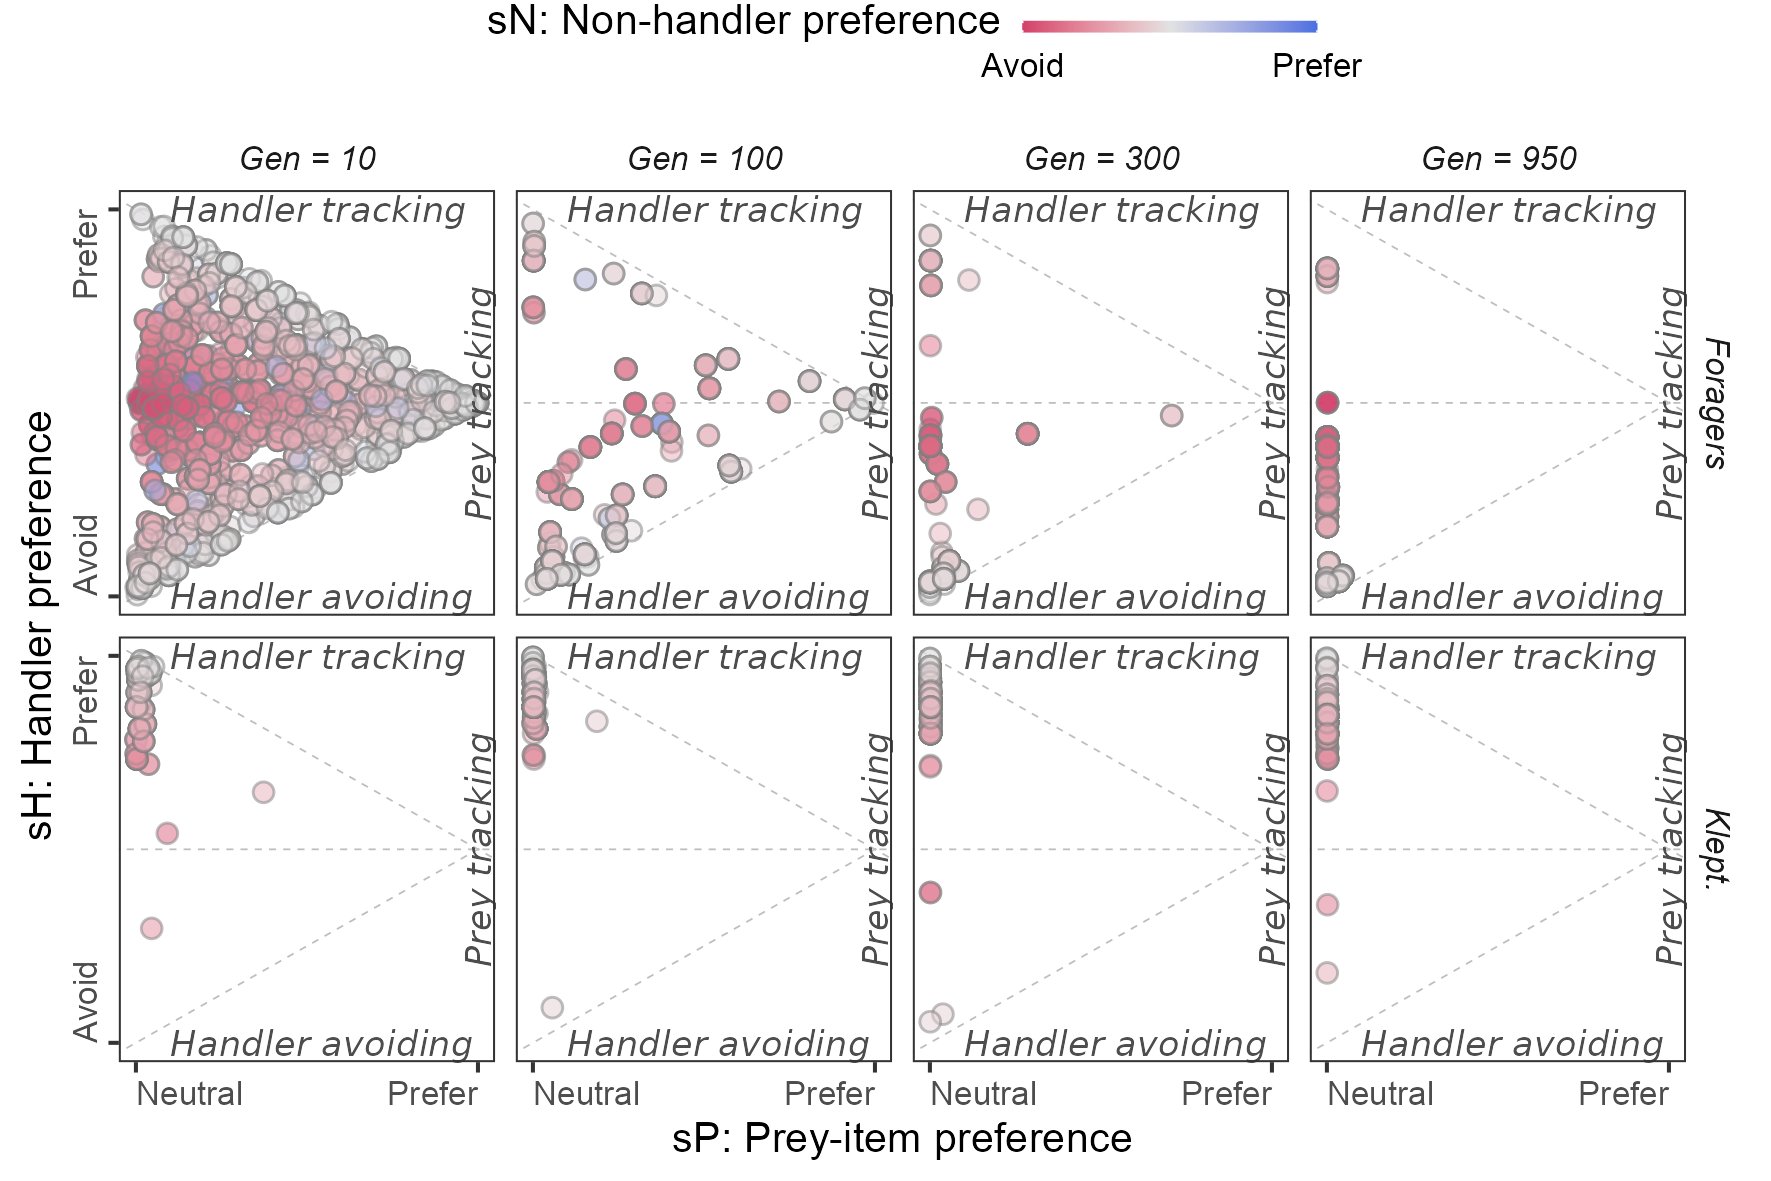
\includegraphics[width=0.85\textwidth]{figures/fig_03.png}
    \caption{
        Model 2 populations with both exploitation competition, and kleptoparasitism as a fixed, inherited strategy reach an \textbf{(A)} activity budget and \textbf{(B)} total intake equlibrium rapidly.
        The initial handling and intake spike is due to very successful handling on undepleted resource landscapes.
        The frequency of stealing activities (red line; panel A) is less than the proportion of kleptoparasitic individuals (orange line; panel A), as successful kleptoparasites are counted as handlers while processing prey items.
        \textbf{(C)} The sustained extraction of prey-items results in an initially rapid depletion of the resource landscape within 10 generations. 
        With a reduction in foraging and handling due to increased stealing after generation 30 (panel A), prey-item depletion is reduced, and the resource landscape recovers.
        The number of individuals on occupied cells is shown as black circles (size = number of individuals). Panels \textbf{A, B} show three replicates, while panel \textbf{C} shows a single replicate; all panels are for $r_{max}$ = 0.01.
    }
    \label{Fig:Model2}
\end{figure}

\begin{figure}[h!]
    \centering
    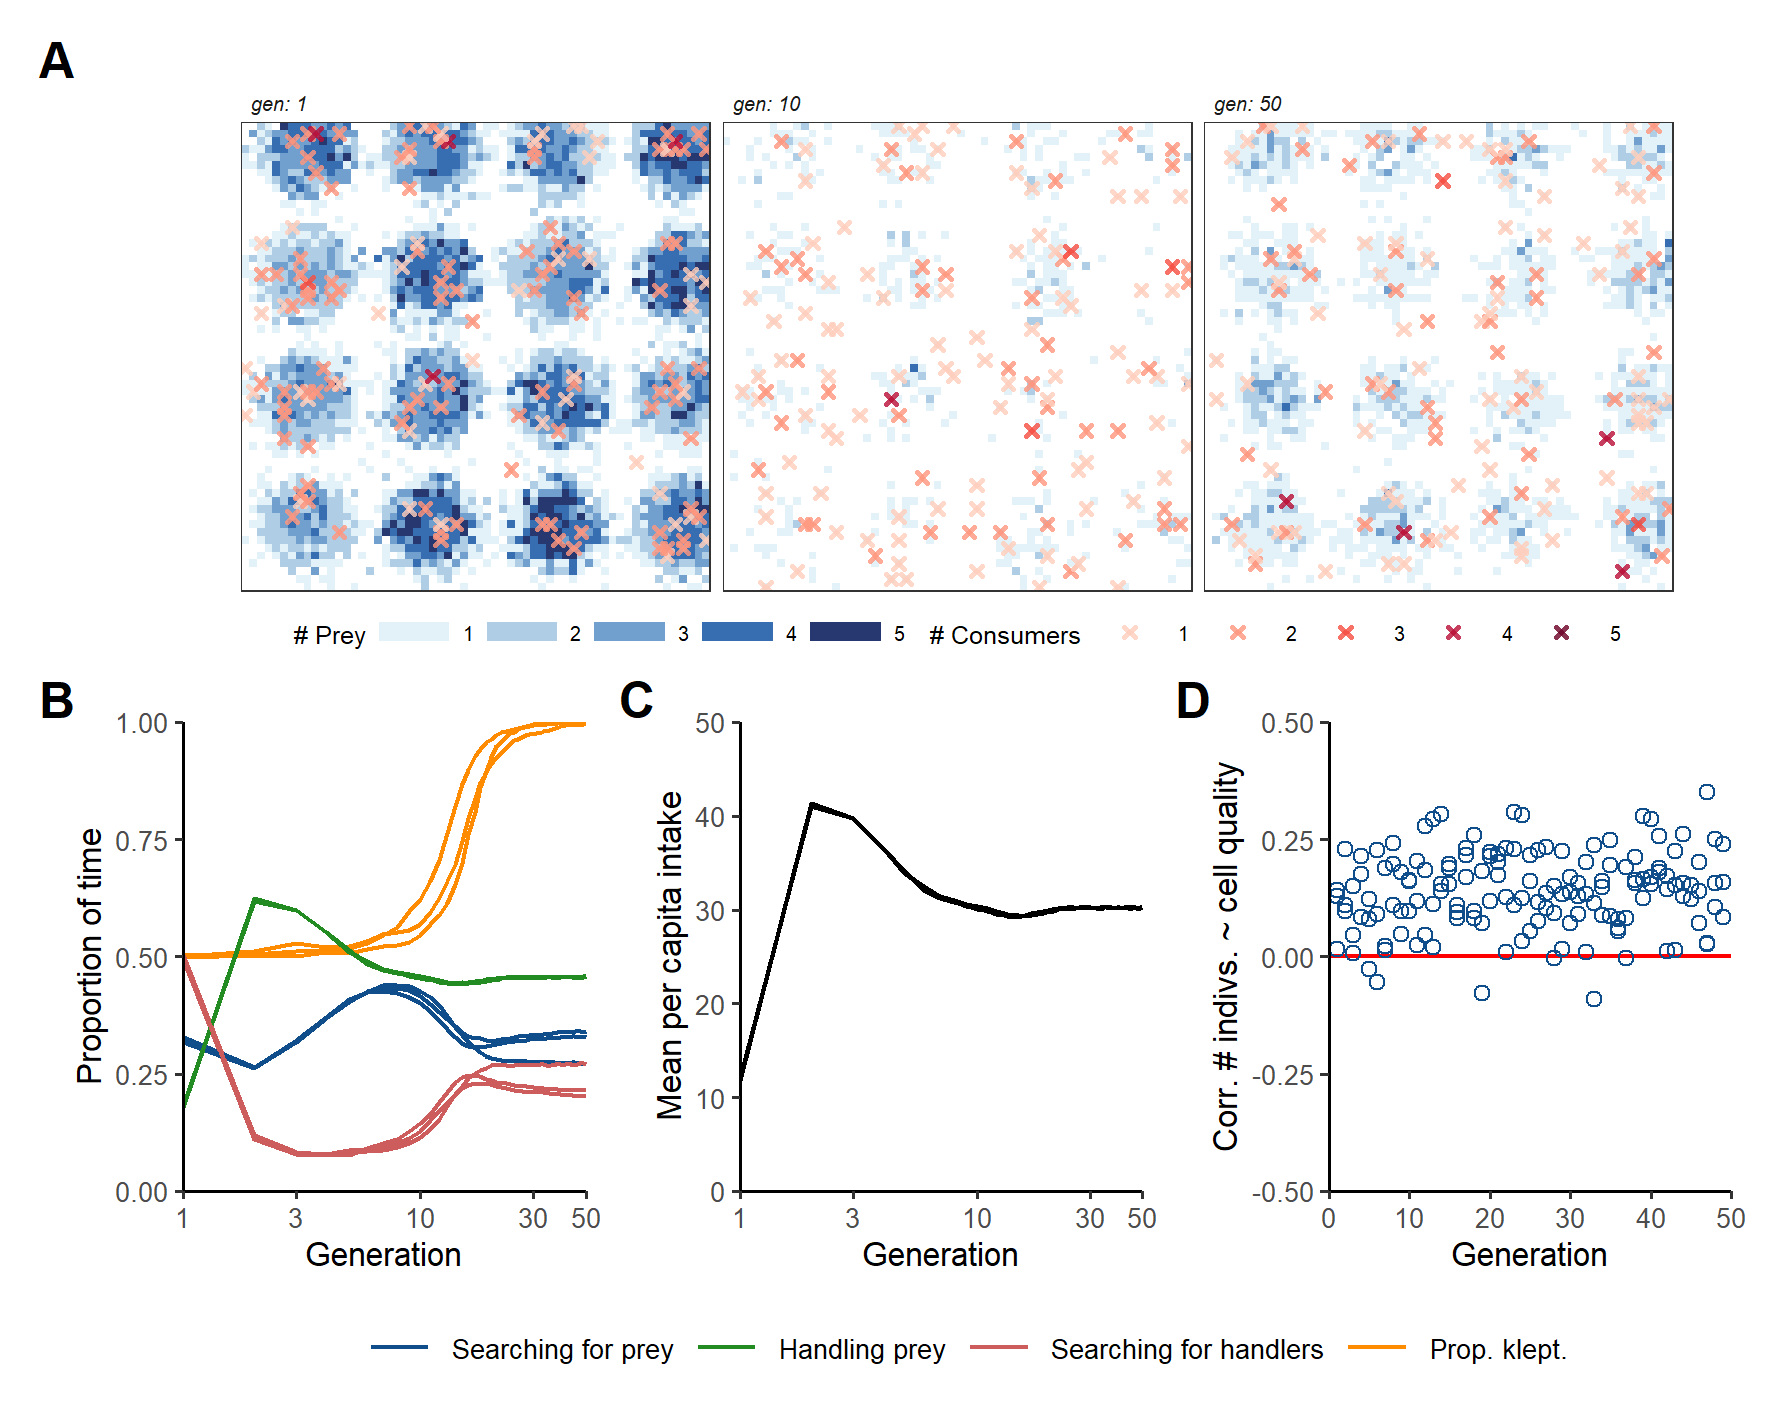
\includegraphics[width=0.85\textwidth]{figures/fig_04.png}
    \caption{
        Model 3 populations with both exploitation competition, and kleptoparasitism as strategy conditional on local cues, reach an \textbf{(A)} activity budget and \textbf{(B)} total intake equlibrium rapidly.
        The initial handling and intake spike is due to very successful handling on undepleted resource landscapes.
        A kleptoparasitic response to handlers (orange line; panel A) becomes rapidly fixed in the population, but the frequency of stealing remains relatively much lower (red line; panel A).
        \textbf{(C)} The sustained extraction of prey-items results in an initially rapid depletion of the resource landscape within 10 generations; the resource landscape regenerates prey-items as kleptoparasitism reduces foraging activities.
        The number of individuals on occupied cells is shown as black circles (size = number of individuals). Panels \textbf{A, B} show three replicates, while panel \textbf{C} shows a single replicate; all panels are for $r_{max}$ = 0.01.
    }
    \label{Fig:Model3}
\end{figure}

\begin{figure}[h!]
    \centering
    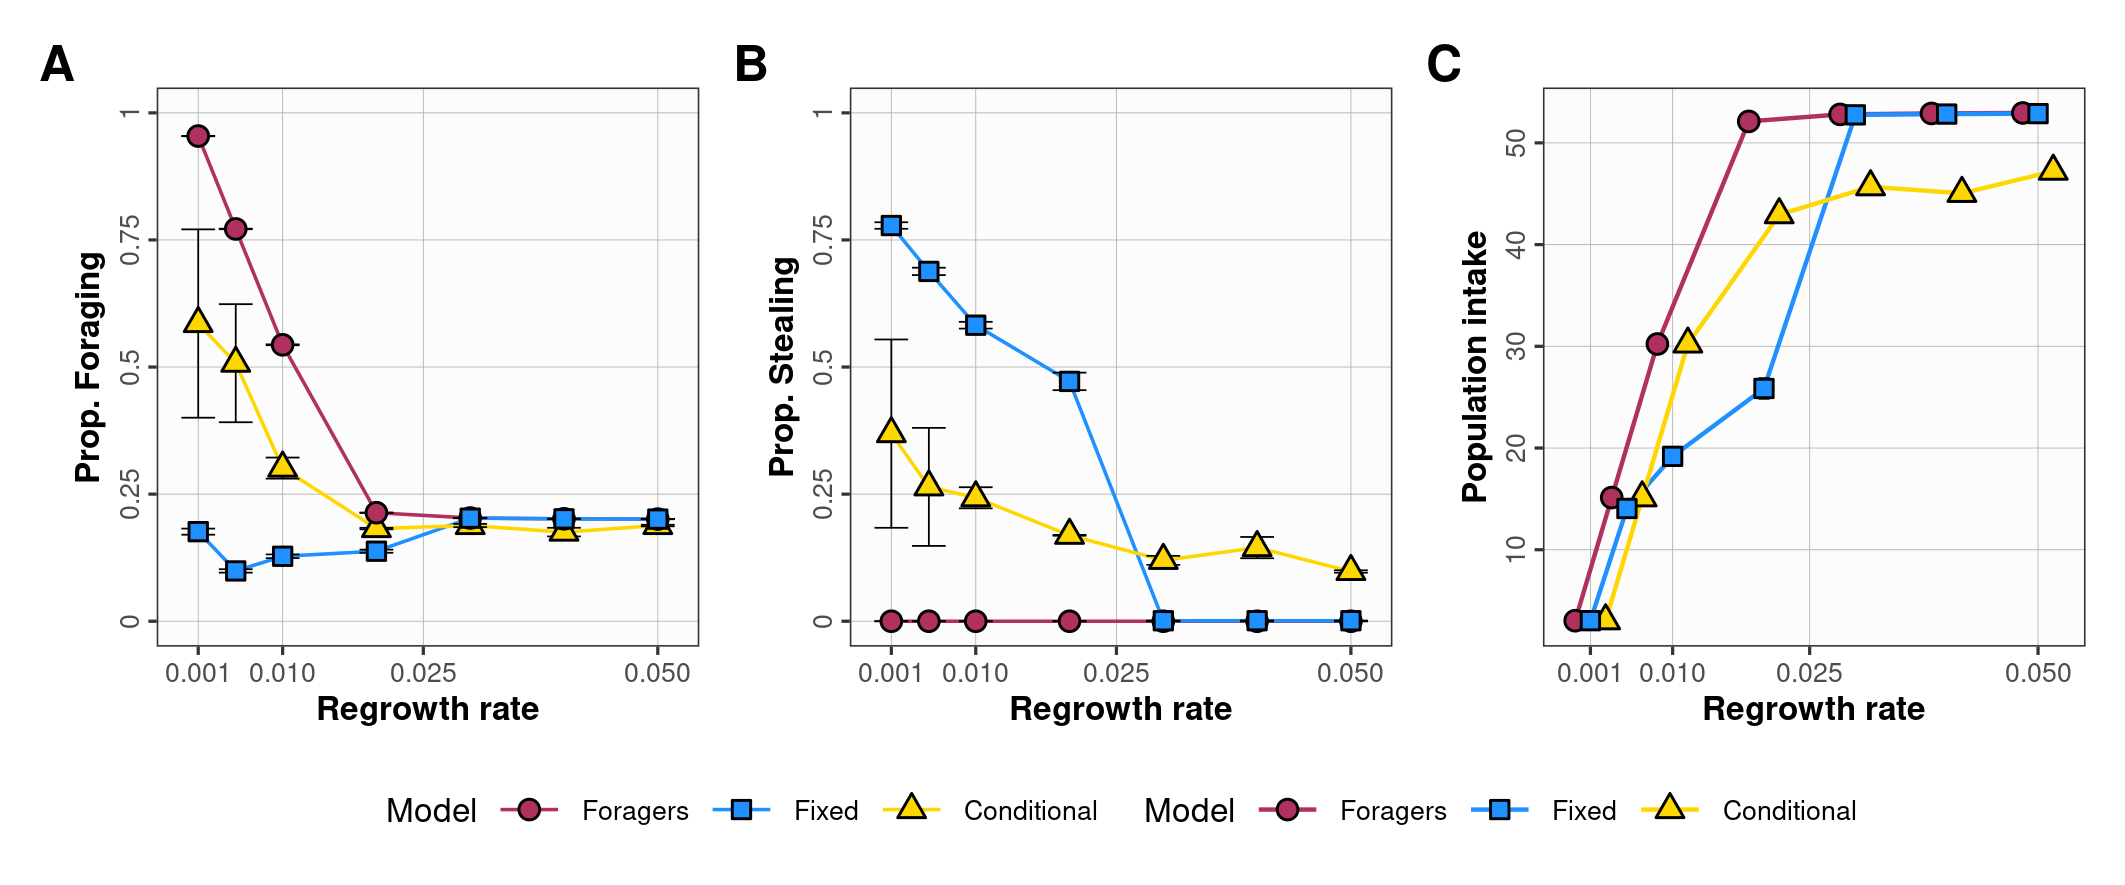
\includegraphics[width=0.85\textwidth]{figures/fig_06.png}
    \caption{Landscape productivity strongly affects model outcomes.
    \textbf{(A)} The frequency foraging reduces with increasing $r_{max}$ in models 1 and 3, but remains relatively stable in model 2. In all three models, this is partly due to an increase in handling caused by increased resoure availability, and \textbf{(B)} partly due to reduced kleptoparasitism in models 2 and 3. In model 2, kleptoparasitism goes extinct at higher $r_{max}$, and such model 2 populations are functionally identical with model 1 populations.
    \textbf{(C)} At low $r_{max}$, populations in all three models achieve similar intakes. At intermediate $r_{max}$ however, popualtions with a conditional kleptoparasitic strategy outperform populations with fixed strategies. At high $r_{max}$, conditional kleptoparasitism populations (model 3) achieve lower intakes than populations in models 1 and 2, which are then functionally identical.
    }
    \label{Fig:Sensitivity}
\end{figure}

\begin{figure}[h!]
    \centering
    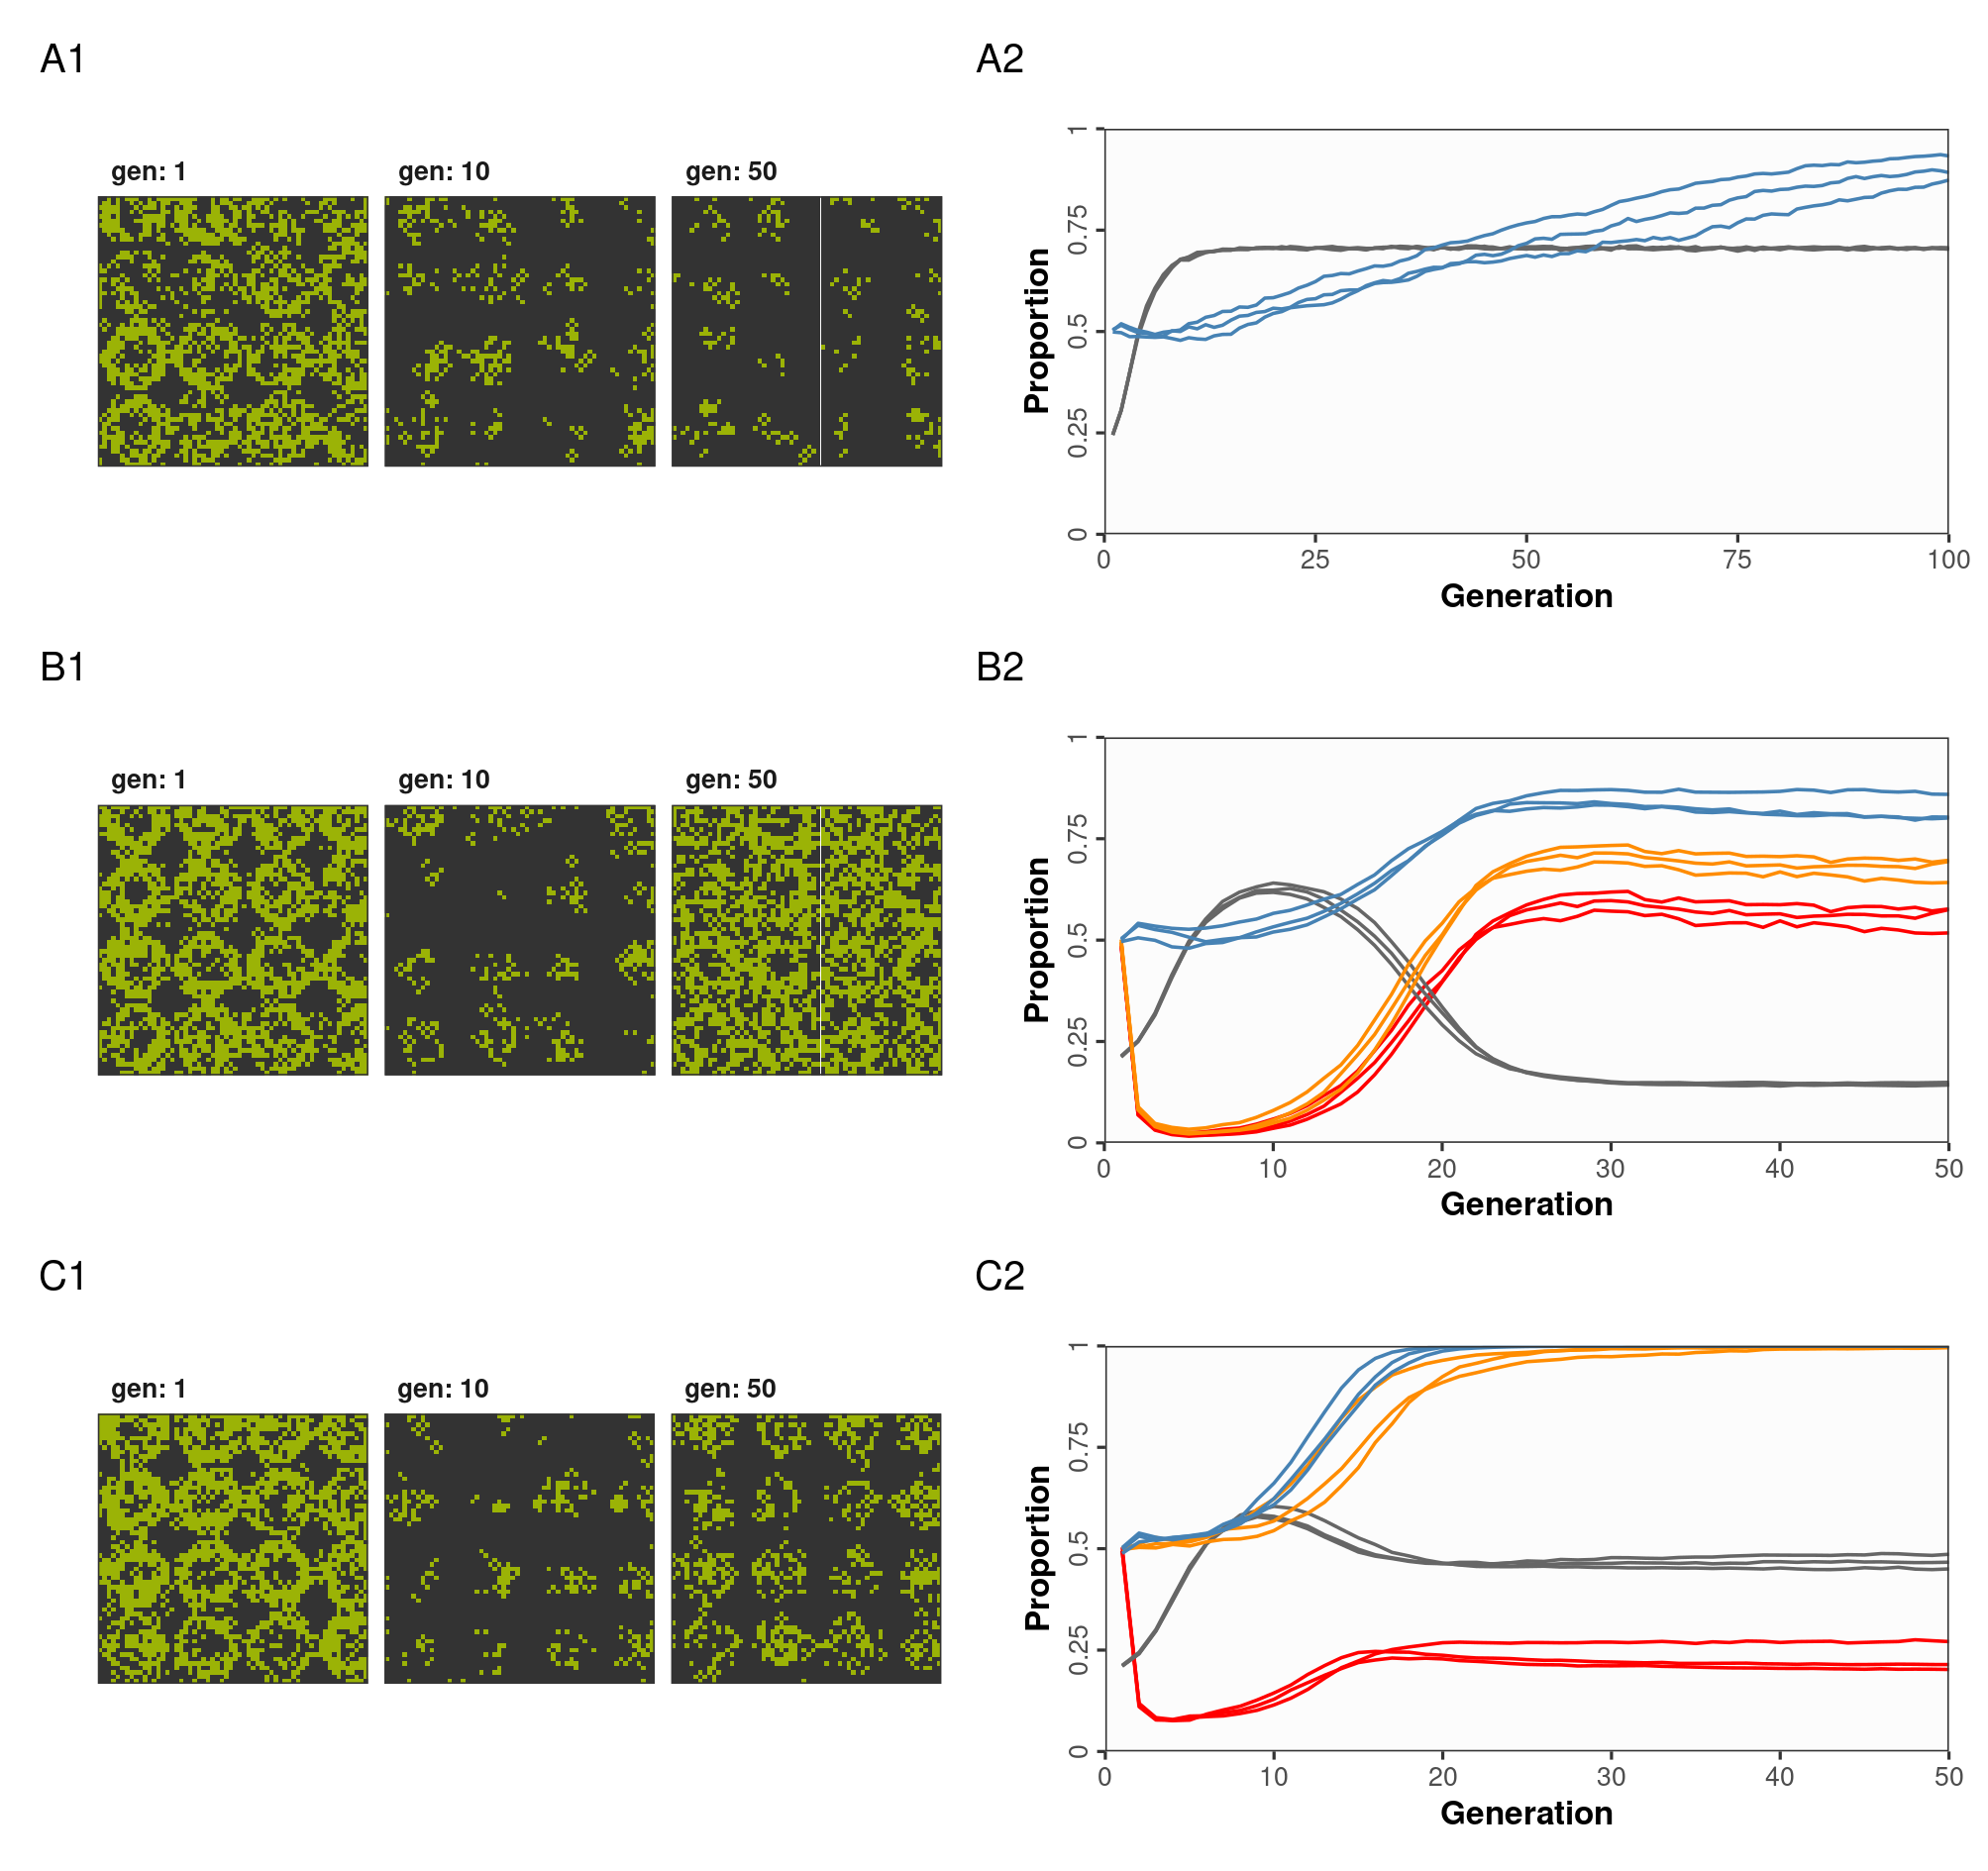
\includegraphics[width=0.90\textwidth]{figures/fig_08.png}
    \caption{
        The evolution and persistence of a kleptoparasitic response (orange lines) and stealing events (red lines) reduces item depletion (coloured cells; row 2), thus reducing `clueless plateaus' (black lines and areas; row 3). All scenarios are shown at $r_{max}$ = 0.01, and only a part of the landscape is shown.
        \textbf{(A, D)} Strong depletion of the resource landscape in Model 1 leads to large areas with no item gradient (clueless plateaus; [D]; black areas; green areas = detectable item gradient).
        \textbf{(B, E)} The emergence and persistence of fixed kleptoparasitism in model 2 leads to a reduction in the area of clueless plateaus within 40 generations ([E]; black areas).
        \textbf{(C, F)} In model 3, the conditional kleptoparasitic strategy leads to depletion intermediate between models 1 and 2, and a similarly intermediate proportion of clueless plateaus on the landscape ([F]).
    }
    \label{Fig:CluelessLandscape}
\end{figure}

\begin{figure}[h!]
    \centering
    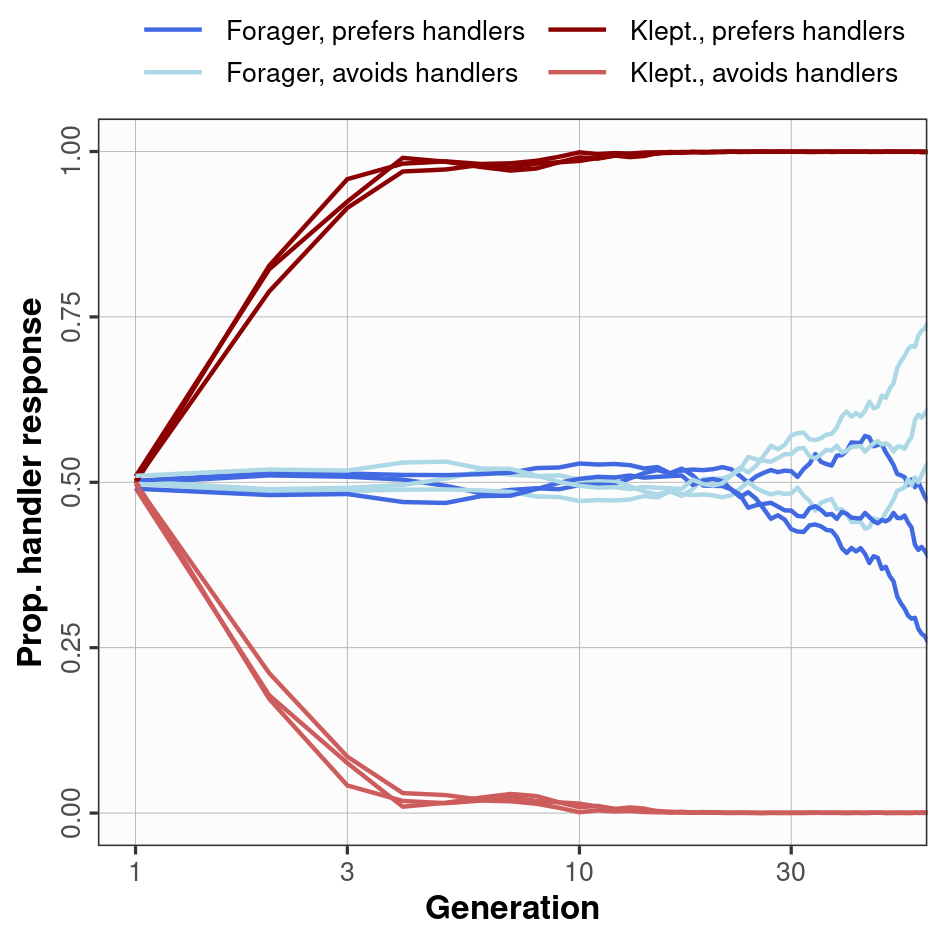
\includegraphics[width=0.85\textwidth]{figures/fig_07.png}
    \caption{
       Movement rules rapidly diverge between fixed behavioural strategies in model 2.
       \textbf{(A)} Within 5 generations, all kleptoparasitic individuals ($\sim$75\% of the population at equilibrium; see Fig. 3A) have an evolved preference for moving towards handlers.
       However, forager individuals are agnostic to handlers, and are equally split between handler preference and avoidance.
       \textbf{(B)} The strong selection on kleptoparasites for moving towards handlers, and the lack of similar selection pressure on foragers, results in the majority of handler preferring individuals in the population being kleptoparasites.
       Both panels show three replicates at $r_{max}$ = 0.01.
    }
    \label{Fig:Syndrome}
\end{figure}



% \subsection{Online figure legends}

% \renewcommand{\thefigure}{A\arabic{figure}}
% \setcounter{figure}{0}

% % \begin{figure}[h!]
% % %\includegraphics{jumps20m}
% % \caption{\textit{A}, the quick red fox proceeding to jump 20~m straight into the air over not one, but several lazy dogs. \textit{B}, the quick red fox landing gracefully despite the skepticism of naysayers.}
% % \label{Fig:Jumps}
% % \end{figure}

% % \begin{figure}[h!]
% % %\includegraphics{jumps20m}
% % \caption{The quicker the red fox jumps, the likelier it is to land near an okapi. For further details, see \citet{LemKapEx07}.}
% % \label{Fig:JumpsOk}
% % \end{figure}

% \renewcommand{\thefigure}{B\arabic{figure}}
% \setcounter{figure}{0}

\end{document}
